\documentclass[tikz,border=10pt]{standalone}
\usepackage{amsmath}
\usepackage[utf8]{inputenc}
\usetikzlibrary{decorations.pathreplacing, arrows.meta, calc, angles, quotes}

\begin{document}
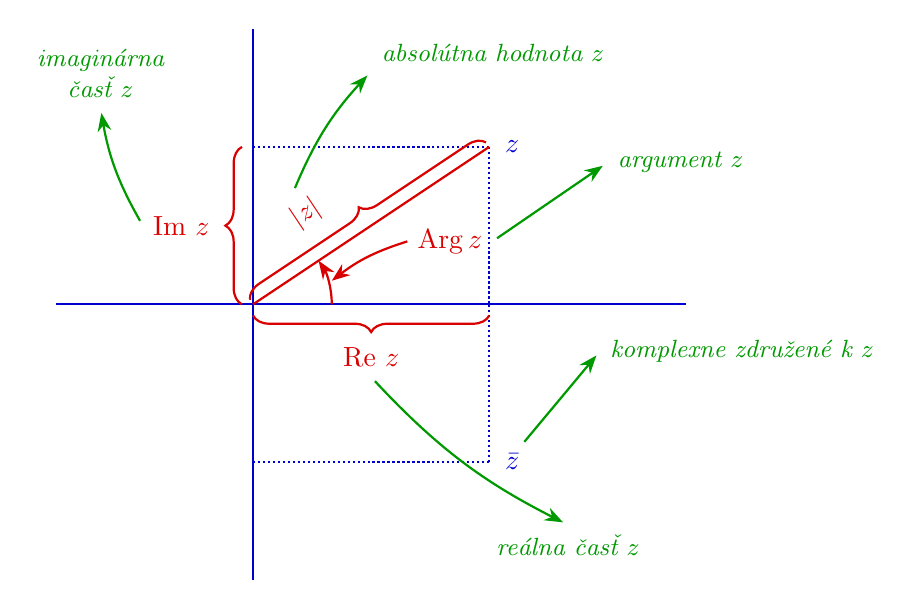
\begin{tikzpicture}[>=Stealth, thick]

    % Define styles
    \tikzset{
        axisline/.style={blue!80!black},
        guide/.style={blue!80!black, densely dotted},
        redpath/.style={red!85!black, thick},
        redarrow/.style={->, red!85!black},
        greenarrow/.style={->, green!60!black, shorten >=2pt, shorten <=2pt},
        bluetext/.style={blue!80!black},
        redtext/.style={red!85!black},
        greentext/.style={green!60!black, font=\small\itshape, align=center},
        brace/.style={decorate, decoration={brace, amplitude=6pt, raise=4pt}, red!85!black},
        brace mirror/.style={decorate, decoration={brace, mirror, amplitude=6pt, raise=4pt}, red!85!black}
    }

    % 1. Define Coordinates
    \coordinate (O) at (0,0);
    \def\xa{3}
    \def\yb{2}
    
    \coordinate (Z) at (\xa, \yb);          % Point z
    \coordinate (Zbar) at (\xa, -\yb);      % Point z_bar (conjugate)
    \coordinate (XPoint) at (\xa, 0);       % Projection on x-axis

    % 2. Axes
    \draw[axisline] (-2.5,0) -- (5.5,0);
    \draw[axisline] (0,-3.5) -- (0,3.5);

    % 3. Z Elements (Upper Half)
    \draw[guide] (Z) -- (XPoint);
    \draw[guide] (Z) -- (0, \yb);
    \draw[redpath] (O) -- (Z);
    \node[bluetext, right, xshift=2pt] at (Z) {$z$};

    % 4. Z_bar Elements (Lower Half - New)
    % Guide lines for z_bar
    \draw[guide] (Zbar) -- (XPoint);
    \draw[guide] (Zbar) -- (0, -\yb);
    % Vector mirroring z
    %\draw[redpath] (O) -- (Zbar);
    % Node label
    \node[bluetext, right, xshift=2pt] at (Zbar) {$\bar{z}$};
    
    % Formula for z_bar placed near the node
    %\node[bluetext, anchor=north west, align=left] at ($(Zbar) + (0.1, 0)$) {$\bar{z} = \text{Re } z - (\text{Im } z) \cdot i$};

    % 5. Braces (Red)
    % Re z (horizontal, mirror to be below)
    \draw[brace mirror] (O) -- (XPoint) node[midway, below=12pt, redtext] (ReZ) {$\text{Re } z$};

    % Im z (vertical, standard to be on left)
    \draw[brace] (0,0) -- (0,\yb) node[midway, left=12pt, redtext] (ImZ) {$\text{Im } z$};

    % |z| (diagonal along vector)
    \draw[brace, decoration={raise=2pt}] (O) -- (Z) node[midway, above left=8pt, redtext, sloped] (AbsZ) {$|z|$};

    % 6. Angle (Argument)
    \pic [draw=red!85!black, ->, angle radius=1.0cm] {angle = XPoint--O--Z};
    
    % Label for argument with arrow
    \node[redtext] (ArgLabel) at (2.5, 0.8) {$\mathrm{Arg}\,z$};
    \draw[redarrow, bend right=10] (ArgLabel.west) to (1.0, 0.3);

    % 7. Green Annotations
    % Absolutna hodnota
    \node[greentext, anchor=west] (AbsText) at (1.5, 3.2) {absolútna hodnota $z$};
    \draw[greenarrow] (AbsZ.north) to [bend left=10] (AbsText.south west);

    % Argument z
    \node[greentext, anchor=west] (ArgText) at (4.5, 1.8) {argument $z$};
    \draw[greenarrow] (ArgLabel.east) -- (ArgText.west);

    % Imaginarna cast
    \node[greentext, anchor=south east] (ImText) at (-1, 2.5) {imaginárna\\časť $z$};
    \draw[greenarrow] (ImZ.west) to [bend left=10] (ImText.south);

    % Realna cast
    \node[greentext, anchor=north] (ReText) at (4.0, -2.8) {reálna časť $z$};
    \draw[greenarrow] (ReZ.south) to [bend right=10] (ReText.north);
    
    % Absolutna hodnota
    \node[greentext, anchor=west,xshift=40pt,yshift=40pt] (ZbarText) at (Zbar) {komplexne združené k $z$};
    \draw[greenarrow] (Zbar.east)+(0.4,0.2) to (ZbarText.west);

\end{tikzpicture}
\end{document}
